\documentclass[conference]{IEEEtran}
\IEEEoverridecommandlockouts

\usepackage{iftex}
\ifXeTeX % Tectonic/XeLaTeX: Times clone; pdfLaTeX (Overleaf default) keeps IEEEtran's standard Times
  \usepackage{fontspec}
  \setmainfont{texgyretermes}[Extension=.otf, UprightFont=*-regular, BoldFont=*-bold,
    ItalicFont=*-italic, BoldItalicFont=*-bolditalic]
\else
  \usepackage[T1]{fontenc}
\fi
\usepackage{cite}
\usepackage{amsmath,amssymb,amsfonts}
\usepackage{graphicx}
\usepackage{booktabs}
\usepackage{multirow}
\usepackage{array}
\usepackage{xcolor}
\usepackage{url}
\usepackage{tikz}
\usetikzlibrary{positioning,arrows.meta,fit,calc,backgrounds}
\usepackage[hidelinks]{hyperref}

% generated by make_figures.py -- do not edit
\newcommand{\NWin}{339}
\newcommand{\NSess}{18}
\newcommand{\HandOldSessAUC}{0.714}
\newcommand{\HandOldSessEER}{46.8}
\newcommand{\HandOldWinAUC}{0.705}
\newcommand{\HandNewSessAUC}{0.740}
\newcommand{\HandNewWinAUC}{0.728}
\newcommand{\LearnWinAUC}{0.835}
\newcommand{\LearnWinAUCsd}{0.021}
\newcommand{\LearnSessAUC}{0.938}
\newcommand{\LearnSessAUCsd}{0.019}
\newcommand{\LearnSessEER}{16.1}
\newcommand{\LearnSessEERsd}{5.7}
\newcommand{\LearnWinEER}{22.8}
\newcommand{\RecallAI}{84.2}
\newcommand{\RecallLip}{70.4}
\newcommand{\RecallScript}{10.0}
\newcommand{\GenFPR}{3.9}
\newcommand{\ITWSpectraEER}{1.25}
\newcommand{\ITWAasistEER}{42.50}
\newcommand{\ITWAasistLEER}{43.50}
\newcommand{\ITWSpectraFPEER}{1.25}
\newcommand{\ASVSpectraEER}{0.00}
\newcommand{\ASVAasistEER}{1.62}
\newcommand{\OpusEER}{3.00}
\newcommand{\NoiseEER}{7.50}
\newcommand{\RevEER}{27.50}
\newcommand{\RevWPEEER}{26.50}
\newcommand{\LFWAUC}{0.986}
\newcommand{\LFWEER}{3.0}
\newcommand{\LFWAcc}{96.9}
\newcommand{\LFWFlag}{3.6}
\newcommand{\SpkAUC}{0.998}
\newcommand{\SpkEER}{1.8}
\newcommand{\SpkTrials}{2000}
\newcommand{\LatMedian}{1.12}
\newcommand{\LatTail}{2.12}
\newcommand{\LatRTF}{0.75}
\newcommand{\RSS}{2.4}


\begin{document}

\title{TrustHire: Real-Time Multimodal Detection of Synthetic and Impersonated Candidates in Remote Job Interviews}

\author{
\IEEEauthorblockN{Mohammed Zamee Shaikh}
\IEEEauthorblockA{\textit{Dept. of Artificial Intelligence and Data Science}\\
\textit{Name of the Institute}\\
City, India \\
email@institute.edu}
\and
\IEEEauthorblockN{Eashan Salian}
\IEEEauthorblockA{\textit{Dept. of Artificial Intelligence and Data Science}\\
\textit{Name of the Institute}\\
City, India \\
email@institute.edu}
\and
\IEEEauthorblockN{Navya Bhootra}
\IEEEauthorblockA{\textit{Dept. of Artificial Intelligence and Data Science}\\
\textit{Name of the Institute}\\
City, India \\
email@institute.edu}
}

\maketitle

\begin{abstract}
Remote hiring now has to deal with candidates who are not who they claim to be: synthetic talking heads, cloned
voices, stand-in proxies, and applicants reading prepared answers off a second screen. Detectors built for one of
these problems are usually evaluated on studio-quality benchmarks that look little like a webcam interview. We
present TrustHire, a system that watches a live interview over WebRTC, cuts it into 3\,s windows with 50\%
overlap, and scores each window with ten evidence modules covering face forgery, voice spoofing, lip
synchrony, face and voice identity continuity, gaze behaviour, remote photoplethysmography, scene objects,
answer delivery, and consistency with the resume. A calibrated fusion stage turns these into a per-window risk
timeline and a session trust score, and every alert is backed by a visual or acoustic explanation. On public
data, the selected voice-spoofing model reaches \ITWSpectraEER\% equal error rate (EER) on In-the-Wild against
\ITWAasistEER\% for the commonly used AASIST baseline, while degrading sharply in reverberant rooms. On a pilot
set of \NSess{} interview recordings collected by the authors, replacing a FaceForensics++-trained detector with
a general AI-image detector and learning the fusion weights raises session-level AUC from \HandOldSessAUC{} to
\LearnSessAUC{}~$\pm$~\LearnSessAUCsd{}. The full pipeline runs at \LatMedian\,s per window on a laptop CPU, faster
than the 1.5\,s hop. We report where the system fails, most notably on scripted reading.
\end{abstract}

\begin{IEEEkeywords}
deepfake detection, voice anti-spoofing, multimodal fusion, remote hiring, audio-visual synchrony, identity verification
\end{IEEEkeywords}

% =====================================================================================================
\section{Introduction}

Video interviews have become the default first round of hiring, and the trust that used to come from sitting in
the same room has not been replaced by anything comparable. In 2022 the FBI warned that applicants were using
deepfake video and stolen identities to win remote technical roles~\cite{fbi2022}. Since then, text-to-video
avatar services and few-shot voice cloning have made convincing fakes cheaper still. Fraud in interviews is
also not only a deepfake problem: a different person can take the call after a genuine applicant has been
verified, or a real candidate can read answers written by someone else.

Most published detectors address a single modality and are tested on curated datasets such as
FaceForensics++~\cite{rossler2019ffpp} or ASVspoof~\cite{wang2020asvspoof}. A recurring finding is that their
accuracy drops once the test data comes from somewhere else~\cite{muller2022itw,yan2023deepfakebench}. An
interviewer, meanwhile, needs something different from a benchmark score: a running indication of
\emph{when} something looks wrong, \emph{which} signal raised the concern, and how sure the system is.

This paper describes TrustHire, a working system built around that need, and the measurements we made while
building it. Our contributions are:
\begin{itemize}
\item a streaming architecture that analyses live WebRTC video and audio in overlapping 3\,s windows with ten
evidence modules, each reporting a score \emph{and} a confidence, so missing or unreliable evidence (no face, no
speech, heavy noise) is handled explicitly rather than imputed;
\item a component study on public data, including a robustness analysis showing that a strong speech
anti-spoofing model fails under room reverberation and that neither front-end dereverberation nor augmentation-based
fine-tuning fixed it;
\item an interview-shaped pilot evaluation in which the commonly used face-forgery model turned out to be
anti-correlated with the ground truth, a general AI-image detector separated real and generated videos, and a
learned, calibrated fusion improved session-level detection; we also show how isotonic calibration on small
folds silently destroyed ranking performance;
\item engineering measures that bring the full pipeline below real time on a CPU-only laptop.
\end{itemize}

% =====================================================================================================
\section{Related Work}

\textit{Face forgery detection.} Frame-level CNNs such as XceptionNet~\cite{chollet2017xception} and
EfficientNet~\cite{tan2019efficientnet} trained on FaceForensics++~\cite{rossler2019ffpp} remain standard
baselines. DeepfakeBench~\cite{yan2023deepfakebench} compared many detectors under a common protocol and
found that accuracy falls sharply once a model trained on one corpus is tested on another, for instance
Celeb-DF~\cite{li2020celebdf} or DFDC~\cite{dolhansky2020dfdc}.
Detectors trained on many generative models, for example linear probes over CLIP features~\cite{ojha2023universal},
generalise better to fully synthetic images, which is closer to the avatars produced by current text-to-video
tools.

\textit{Voice anti-spoofing.} AASIST~\cite{jung2022aasist} and RawNet2~\cite{tak2021rawnet2} operate on raw
waveforms and perform very well on ASVspoof 2019 LA~\cite{wang2020asvspoof}. M\"uller et al.~\cite{muller2022itw}
showed that such models break down on In-the-Wild recordings of public figures. Putting a self-supervised
encoder in front of the classifier, XLS-R~\cite{babu2022xlsr} being a common choice, closes much of this gap; the Spectra-0
model~\cite{spectra0} we use combines XLS-R with an ECAPA-TDNN head.

\textit{Audio-visual consistency.} SyncNet~\cite{chung2016syncnet} learns a joint embedding of mouth crops and
MFCC frames and estimates the audio-visual offset; AV-HuBERT~\cite{shi2022avhubert} learns stronger joint
representations at a much higher compute cost. Multimodal deepfake datasets such as
FakeAVCeleb~\cite{khalid2021fakeavceleb} and LAV-DF~\cite{cai2022lavdf} combine visual and audio manipulations.

\textit{Identity and liveness.} ArcFace~\cite{deng2019arcface} with SCRFD detection~\cite{guo2022scrfd} and
ECAPA-TDNN~\cite{desplanques2020ecapa} are widely used for face and speaker verification. Remote
photoplethysmography methods such as CHROM~\cite{dehaan2013chrom} and POS~\cite{wang2017pos} recover a pulse
signal from skin colour and have been used as liveness cues.

To our knowledge, prior work rarely combines these signals in a single streaming system aimed at interviews or
evaluates them on interview-like recordings, which is the gap this work targets. Multimodal fusion in general is
surveyed in~\cite{baltrusaitis2019multimodal}.

% =====================================================================================================
\section{System Design}

\begin{figure*}[t]
\centering
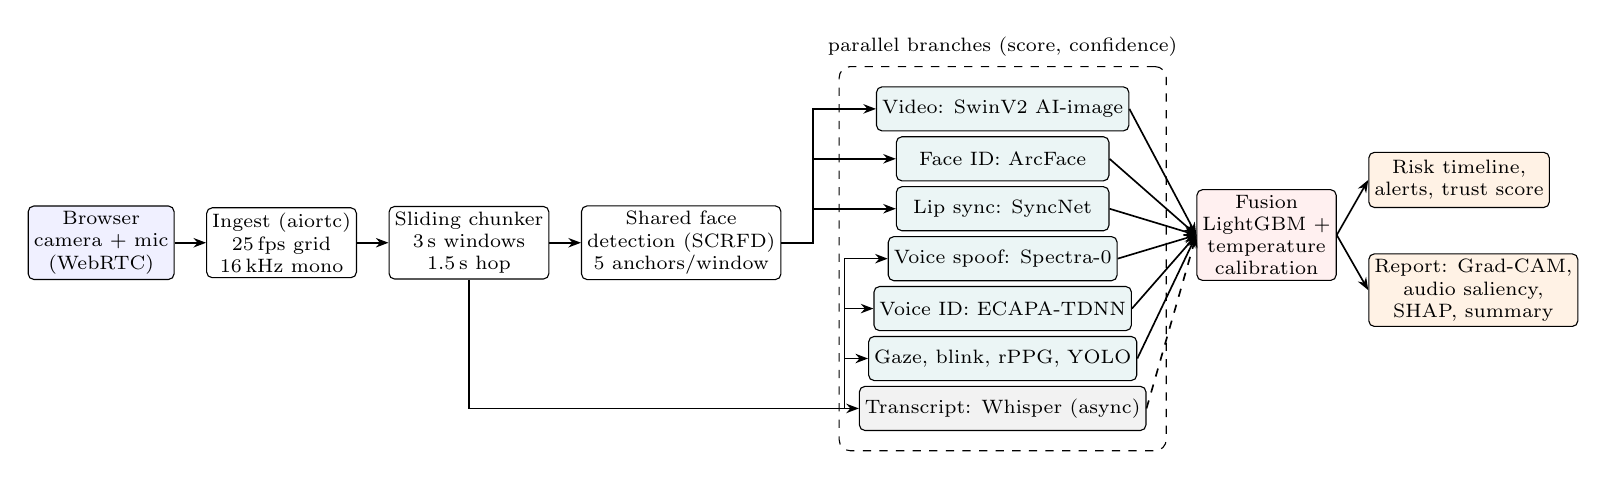
\begin{tikzpicture}[
  font=\scriptsize, node distance=3mm and 4mm,
  box/.style={draw, rounded corners=2pt, align=center, minimum height=7mm, inner sep=2pt, fill=white},
  src/.style={box, fill=blue!6},
  mod/.style={box, fill=teal!8, minimum width=27mm, minimum height=5.6mm},
  outbox/.style={box, fill=orange!10},
  arr/.style={-{Stealth[length=1.6mm]}, semithick}]
  \node[src] (browser) {Browser\\camera + mic\\(WebRTC)};
  \node[box, right=of browser] (ingest) {Ingest (aiortc)\\25\,fps grid\\16\,kHz mono};
  \node[box, right=of ingest] (chunk) {Sliding chunker\\3\,s windows\\1.5\,s hop};
  \node[box, right=of chunk] (face) {Shared face\\detection (SCRFD)\\5 anchors/window};
  \node[mod, right=12mm of face, yshift=17mm] (v) {Video: SwinV2 AI-image};
  \node[mod, below=0.6mm of v] (fid) {Face ID: ArcFace};
  \node[mod, below=0.6mm of fid] (sync) {Lip sync: SyncNet};
  \node[mod, below=0.6mm of sync] (as) {Voice spoof: Spectra-0};
  \node[mod, below=0.6mm of as] (vid) {Voice ID: ECAPA-TDNN};
  \node[mod, below=0.6mm of vid] (beh) {Gaze, blink, rPPG, YOLO};
  \node[mod, below=0.6mm of beh, fill=gray!10] (tr) {Transcript: Whisper (async)};
  \node[box, right=10mm of as, yshift=3mm, fill=red!6] (fuse) {Fusion\\LightGBM +\\temperature\\calibration};
  \node[outbox, right=of fuse, yshift=7mm] (tl) {Risk timeline,\\alerts, trust score};
  \node[outbox, right=of fuse, yshift=-7mm] (rep) {Report: Grad-CAM,\\audio saliency,\\SHAP, summary};
  \begin{scope}[on background layer]
    \node[draw, dashed, rounded corners, fit=(v)(tr), inner sep=2.5mm, label={[font=\scriptsize]above:{parallel branches (score, confidence)}}] (br) {};
  \end{scope}
  \draw[arr] (browser) -- (ingest);
  \draw[arr] (ingest) -- (chunk);
  \draw[arr] (chunk) -- (face);
  \foreach \n in {v,fid,sync} \draw[arr] (face.east) -- ++(4mm,0) |- (\n.west);
  \coordinate (abus) at ($(face.east)+(8mm,0)$);
  \draw[semithick] (chunk.south) |- (abus |- tr.west);
  \foreach \n in {as,vid,beh,tr} \draw[arr] (abus |- tr.west) -- (abus |- \n.west) -- (\n.west);
  \foreach \n in {v,fid,sync,as,vid,beh} \draw[arr] (\n.east) -- (fuse.west);
  \draw[arr, dashed] (tr.east) -- (fuse.west);
  \draw[arr] (fuse.east) -- (tl.west);
  \draw[arr] (fuse.east) -- (rep.west);
\end{tikzpicture}
\caption{TrustHire architecture. Each window is analysed by parallel branches that share face detections; each
branch returns a score in $[0,1]$ and a confidence. The transcript branch runs asynchronously and updates earlier
windows when an answer has been transcribed.}
\label{fig:arch}
\end{figure*}

\subsection{Streaming pipeline}

The browser sends camera and microphone streams over WebRTC to a FastAPI server, where an aiortc receiver resamples
video onto a constant 25\,fps grid (needed by SyncNet) and audio to 16\,kHz mono (Fig.~\ref{fig:arch}). Video frames
are spaced using the sender's RTP clock rather than their arrival time. We found this mattered: with arrival-time
stamps, bursty delivery under CPU load scrambled the lip motion and SyncNet's confidence fell from about 8 to below 2 on
a clip that was perfectly synchronised offline. A chunker emits 3\,s windows every 1.5\,s. Results are pushed to a
React dashboard over a WebSocket; recorded interviews follow the same path through an offline job queue.

\subsection{Evidence modules}

Table~\ref{tab:modules} lists the modules. All of them report a risk $s_m\in[0,1]$, where higher means more suspicious,
together with a confidence $c_m\in[0,1]$ that reflects the quality of the evidence: face size and coverage for the video
branches, the fraction of speech found by voice activity detection, and an estimated speech-to-noise ratio for the
anti-spoofing branch. A module with nothing to measure returns $c_m=0$ and is treated as missing.

\begin{table}[t]
\caption{Evidence modules and the models behind them}
\label{tab:modules}
\centering
\scriptsize
\setlength{\tabcolsep}{3pt}
\renewcommand{\arraystretch}{1.1}
\begin{tabular}{@{}>{\raggedright}p{1.45cm}>{\raggedright}p{3.45cm}>{\raggedright\arraybackslash}p{2.95cm}@{}}
\toprule
Module & Model & What it flags \\
\midrule
Video forgery & SwinV2-L AI-image classifier~\cite{liu2022swinv2,aiimagedetector} & generated / swapped faces \\
Voice spoofing & Spectra-0 (XLS-R + ECAPA)~\cite{spectra0} & synthetic or converted speech \\
Lip synchrony & SyncNet~\cite{chung2016syncnet} & dubbed or misaligned audio \\
Face identity & SCRFD + ArcFace R50~\cite{guo2022scrfd,deng2019arcface} & person changed after enrolment \\
Voice identity & ECAPA-TDNN~\cite{desplanques2020ecapa} & speaker changed \\
Behaviour & MediaPipe Face Mesh~\cite{kartynnik2019facemesh} & off-screen gaze, reading sweeps \\
Liveness & rPPG, POS + CHROM~\cite{wang2017pos,dehaan2013chrom} & absent pulse signal \\
Scene objects & YOLO26n (COCO) & phone, second person, extra screen \\
Answer delivery & Whisper~\cite{radford2023whisper} + prosody & fluency typical of reading \\
Resume check & embedding retrieval + NLI & contradictions with the CV \\
\bottomrule
\end{tabular}
\end{table}

Identity continuity compares each window both with the enrolled reference and with a running average of the
session, so it can detect a person who was wrong from the start as well as one who changes mid-interview. Lip
synchrony is scored against the session's own median offset, because genuine set-ups often carry a constant
skew (Bluetooth headsets add 150--250\,ms); offsets larger than 320\,ms remain suspicious regardless.

\subsection{Fusion and calibration}

For each window $t$ the fusion stage receives $\{(s_m,c_m)\}$ for all modules plus a few raw measurements
(sync confidence, identity similarities, speech SNR). We compared three fusers. The first is a
confidence-weighted mean of log-odds with an additional term that lets a single strong module dominate:
\begin{equation}
z_t = b + \frac{\sum_m w_m c_m \ell_m}{\sum_m w_m c_m} + \sum_m v_m c_m \max(0,\ell_m),
\end{equation}
where $\ell_m=\operatorname{logit}(s_m)$ and the weights $w_m, v_m \ge 0$ are fitted by logistic loss.
The mean term stops correlated modules that all report ``genuine'' from compounding into unrealistic certainty, a
problem we saw with a plain naive-Bayes sum. The second fuser is a LightGBM stacker~\cite{ke2017lightgbm} over scores,
confidences, raw measurements and rolling statistics of the previous five windows, which handles missing modules
natively. The third is a small transformer that treats each module in the current and three previous windows as a
token and is trained with random modality dropout. Outputs are calibrated with temperature
scaling~\cite{guo2017calibration} fitted on held-out participants. The session trust score is
$100\,(1-R)$ with $R = 0.6\,\overline{r}_{\text{top}10\%} + 0.4\,\overline{r}$, so a short burst of strong
evidence matters while one noisy window does not decide the outcome.

\subsection{Explanations}

Every alert links to its evidence. For the video branch we compute Grad-CAM~\cite{selvaraju2017gradcam} on the
classifier's third stage (Fig.~\ref{fig:gradcam}); for audio, an occlusion map shows which quarter-second slices
raised the spoof probability; for the LightGBM fuser, SHAP values~\cite{lundberg2017shap} give each module's
contribution. A short natural-language summary is generated from these numbers and exported with the timeline as a
PDF report. The report states that it is evidence for a reviewer, not a decision.

\begin{figure}[t]
\centering
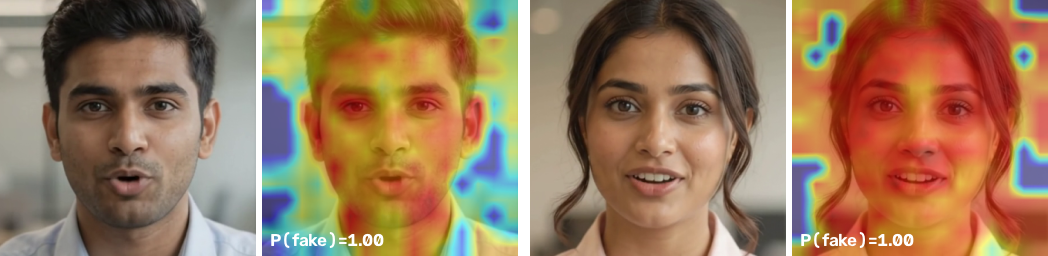
\includegraphics[width=\columnwidth]{figures/gradcam.png}
\caption{Grad-CAM for the video branch on two AI-generated avatars from the pilot set (original and overlay). Only
synthetic faces are shown.}
\label{fig:gradcam}
\end{figure}

\subsection{Running below real time on a CPU}

The deployment target was a laptop without a GPU (Intel Core i5-1235U). A first version needed 9.5\,s per window.
Three changes made the difference (Fig.~\ref{fig:latency}). Flushing denormal floating-point values to zero in ONNX
Runtime made the convolutional models up to forty times faster. Capping each concurrent branch at three threads
removed oversubscription. Finally, because consecutive windows overlap by half, running the most expensive modules
on alternate windows still covers every instant of the interview while halving their cost; in between, the last
result is carried forward. The SwinV2 and Spectra-0 models are additionally quantised to int8, which cut their latency
by factors of 1.9 and 1.6 without changing their accuracy on our evaluation sets.

% =====================================================================================================
\section{Experimental Setup}

\textit{Public data.} Voice anti-spoofing was evaluated on stratified subsets of In-the-Wild~\cite{muller2022itw}
(400 utterances, two shards) and the ASVspoof 2019 LA evaluation set~\cite{wang2020asvspoof} (308 utterances). Each
utterance was scored on its first 4.04\,s, the same context the live system uses. Robustness conditions were applied to
the same utterances: additive white and pink noise, Opus at 16\,kb/s (typical of WebRTC), MP3 at 32\,kb/s, telephone
band-limiting, and synthetic room reverberation with RT$_{60}$ of 0.25--0.7\,s. Face verification used the 1000 LFW test
pairs~\cite{huang2007lfw}, run end-to-end through detection and alignment; speaker verification used \SpkTrials{} trials
of 4\,s segments from LibriSpeech test-clean~\cite{panayotov2015librispeech}.

\textit{Pilot interview set.} The authors recorded \NSess{} videos (\NWin{} analysis windows): five genuine webcam
answers and two re-encoded copies of them (480p and 1440p), three answers read from a prepared script, two clips with
replaced or misaligned audio, and six fully AI-generated talking heads from a text-to-video service. All real footage
shows one consenting participant. The re-encoded copies were placed in the same cross-validation group as their
originals so that no model is tested on a copy of a video it was trained on.

\textit{Protocol and metrics.} We report AUC and EER, recall at a fixed false-positive rate (FPR), and latency. Fusion
models were evaluated with grouped five-fold cross-validation; inside each training fold, a fifth of the groups were held
out to fit the calibrator. Because the pilot set is small, we ran each fusion experiment five times with
different seeds and quote the average together with its spread (mean $\pm$ one SD).

% =====================================================================================================
\section{Results}

\subsection{Voice anti-spoofing and robustness}

Table~\ref{tab:audio} confirms the generalisation gap reported in~\cite{muller2022itw}. AASIST is nearly perfect on
ASVspoof but close to chance on In-the-Wild, whereas Spectra-0 stays near 1\% EER on both. Dynamic int8 quantisation of
Spectra-0 left the EER unchanged and made it 1.7 times faster on our CPU, so the quantised model is deployed.

\begin{table}[t]
\caption{Voice anti-spoofing on public data (EER \%, AUC in brackets)}
\label{tab:audio}
\centering
\scriptsize
\begin{tabular}{@{}lcc@{}}
\toprule
Model & In-the-Wild (n=400) & ASVspoof 2019 LA (n=308) \\
\midrule
AASIST~\cite{jung2022aasist} & \ITWAasistEER{} (0.580) & \ASVAasistEER{} (0.998) \\
AASIST-L~\cite{jung2022aasist} & \ITWAasistLEER{} (0.618) & 2.27 (0.999) \\
Spectra-0~\cite{spectra0} & \ITWSpectraFPEER{} (0.998) & 0.00 (1.000) \\
Spectra-0, int8 (deployed) & \ITWSpectraEER{} (0.998) & \ASVSpectraEER{} (1.000) \\
\bottomrule
\end{tabular}
\end{table}

\begin{figure}[t]
\centering
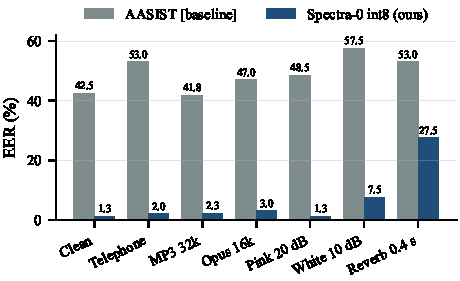
\includegraphics[width=\columnwidth]{figures/audio_robustness.pdf}
\caption{EER on the same In-the-Wild utterances under channel degradations.}
\label{fig:audiorob}
\end{figure}

Codecs cost little and noise a moderate amount (Fig.~\ref{fig:audiorob}): Opus raised the EER to \OpusEER\%, and
white noise at 10\,dB to \NoiseEER\%. Reverberation was a different story. At RT$_{60}=0.4$\,s, typical of an ordinary furnished
room, the EER rose to \RevEER\% and more than a quarter of genuine speakers crossed the 0.5 decision threshold
(Fig.~\ref{fig:reverb}). Two remedies failed. WPE dereverberation~\cite{nakatani2010wpe} in front of the detector gave
\RevWPEEER\% EER. Fine-tuning Spectra-0 for two epochs on ASVspoof 2019 LA with reverberation, noise and codec
augmentation (on a Tesla T4) lowered the EER slightly but shifted the score distribution, so that 54--86\% of
reverberant genuine speakers were flagged. We kept the released model and instead lower this module's confidence
when the estimated speech-to-noise ratio is poor.

\begin{figure}[t]
\centering
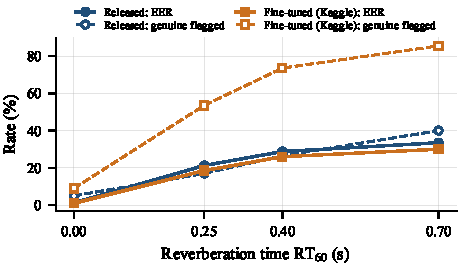
\includegraphics[width=\columnwidth]{figures/reverb_dose.pdf}
\caption{Effect of room reverberation on the voice-spoofing module before and after augmentation-based fine-tuning.
Solid lines: EER. Dashed lines: share of genuine speakers with spoof probability above 0.5.}
\label{fig:reverb}
\end{figure}

\subsection{Identity and lip synchrony}

On LFW the end-to-end face path reached an AUC of \LFWAUC{} and \LFWEER\% EER (accuracy \LFWAcc\%). This is below the
accuracy usually quoted for ArcFace, which is measured on pre-aligned crops; at the deployed similarity threshold no
impostor pair was accepted, and \LFWFlag\% of same-person pairs would be flagged. Speaker verification on LibriSpeech
gave an AUC of \SpkAUC{} and \SpkEER\% EER. For lip synchrony we shifted the audio of a reference talking-head clip by
$-400$ to $+400$\,ms; the estimated offset was within one frame of the truth in every window, and the sync risk rose
monotonically with the shift (Fig.~\ref{fig:desync}). This check uses a single clip and should be read as a sanity test,
not a benchmark.

\begin{figure}[t]
\centering
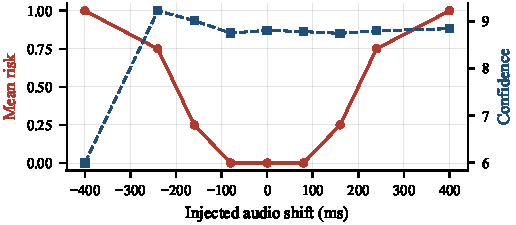
\includegraphics[width=\columnwidth]{figures/desync.pdf}
\caption{Lip-synchrony risk and SyncNet confidence versus an injected audio shift.}
\label{fig:desync}
\end{figure}

\subsection{Pilot interview set}

\textit{Video detector selection.} The DeepfakeBench EfficientNet-B4 trained on FaceForensics++ was, on our recordings,
anti-correlated with the truth: face crops from genuine webcam video received higher fake probabilities than the
AI-generated avatars (Fig.~\ref{fig:detsel}, AUC 0.00). We benchmarked eight publicly available detectors on the same
frames. A SwinV2-L classifier trained to separate AI-generated from real images~\cite{aiimagedetector} gave every real
video a mean fake probability below 0.01 and every generated video one above 0.96. With six generated and twelve real
videos this perfect separation is encouraging but not conclusive, and the set contains no real-time face swaps.

\begin{figure}[t]
\centering
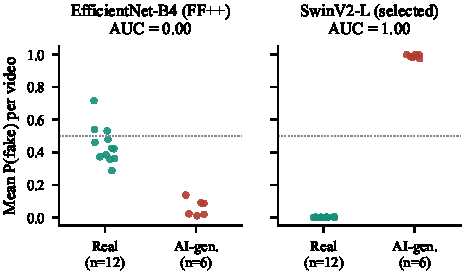
\includegraphics[width=\columnwidth]{figures/detector_selection.pdf}
\caption{Mean per-video fake probability on the pilot set for the FaceForensics++-trained baseline and the selected
detector.}
\label{fig:detsel}
\end{figure}

\textit{Fusion.} With the new video detector and the hand-set fusion weights, genuine videos received trust scores of 95
to 99 and generated videos 0 to 2. Session-level AUC stayed low, however, because audio-mismatch and scripted clips were
scored as genuine. One dubbed clip, for example, obtained a trust score of 97.6 although its lip-sync risk was 0.82,
higher than that of any genuine video; the fixed weights simply gave lip synchrony too little influence. Learning the
weights fixed most of this (Fig.~\ref{fig:roc}). Table~\ref{tab:fusion} summarises the comparison.

\begin{figure}[t]
\centering
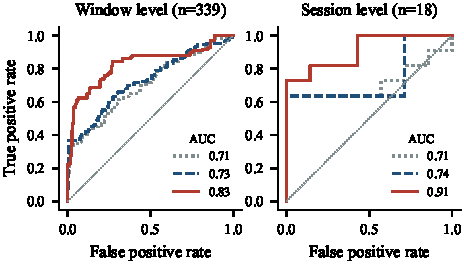
\includegraphics[width=\columnwidth]{figures/roc_fusion.pdf}
\caption{Cross-validated ROC curves on the pilot set (learned fusion shown for one seed).}
\label{fig:roc}
\end{figure}

\begin{table}[t]
\caption{Pilot-set detection, grouped cross-validation}
\label{tab:fusion}
\centering
\scriptsize
\setlength{\tabcolsep}{4pt}
\begin{tabular}{@{}>{\raggedright\arraybackslash}p{2.2cm}ccc@{}}
\toprule
Configuration & Window AUC & Session AUC & Sess.\ EER (\%) \\
\midrule
Hand-set, FF++ & \HandOldWinAUC & \HandOldSessAUC & \HandOldSessEER \\
Hand-set, SwinV2 & \HandNewWinAUC & \HandNewSessAUC & -- \\
Learned (5 seeds) & \LearnWinAUC\,$\pm$\,\LearnWinAUCsd & \LearnSessAUC\,$\pm$\,\LearnSessAUCsd & \LearnSessEER\,$\pm$\,\LearnSessEERsd \\
\midrule
\multicolumn{4}{@{}l}{\textit{Learned fusion, recall at 5\% window FPR (mean of 5 seeds)}} \\
AI-generated & \multicolumn{3}{l}{\RecallAI\%} \\
Audio mismatch & \multicolumn{3}{l}{\RecallLip\%} \\
Scripted reading & \multicolumn{3}{l}{\RecallScript\%} \\
Genuine (flagged) & \multicolumn{3}{l}{\GenFPR\%} \\
\bottomrule
\end{tabular}
\end{table}

\textit{Calibration matters for ranking.} Our first learned fuser used isotonic regression~\cite{zadrozny2002isotonic},
fitted on the three or four videos available for calibration in each fold. Isotonic regression is a step function, and
on so few videos it mapped 339 window scores onto only 52 to 112 distinct values. The resulting ties lowered and
destabilised the ranking: over five seeds, session AUC was $0.886\pm0.083$, against \LearnSessAUC~$\pm$~\LearnSessAUCsd{}
with rank-preserving temperature scaling. We now use temperature scaling for every fuser.

\textit{Ablation.} Fig.~\ref{fig:ablation} compares modality subsets. The transcript features hurt every combination
they were part of; on their own they ranked sessions worse than chance. On spoken answers the AI-text detector assigned
probabilities above 0.95 to several genuine responses, and the fluency features overlapped completely between scripted
and spontaneous answers. The deployed fusion therefore excludes transcript features from the score but still shows them
to the reviewer. No module separated scripted reading from genuine answers in this set.

\begin{figure}[t]
\centering
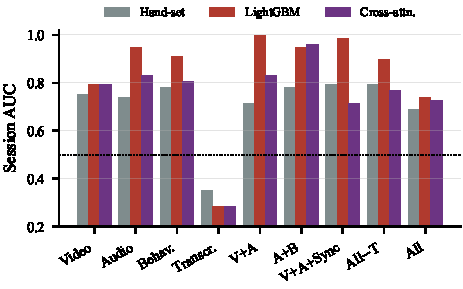
\includegraphics[width=\columnwidth]{figures/ablation.pdf}
\caption{Session-level AUC on the pilot set for modality subsets and fusers (grouped cross-validation).}
\label{fig:ablation}
\end{figure}

\subsection{Latency}

With all modules enabled, the median processing time is \LatMedian\,s per 3\,s window (95th percentile \LatTail\,s), a
real-time factor of \LatRTF, with a peak memory footprint of \RSS\,GB (Fig.~\ref{fig:latency}). The transcript branch is
excluded from this figure because it runs asynchronously when an answer ends.

\begin{figure}[t]
\centering
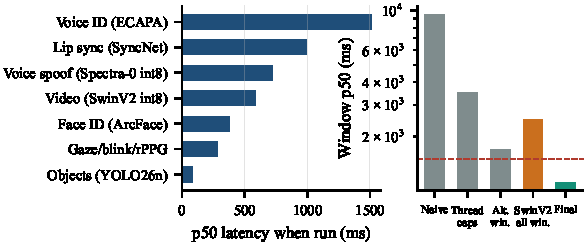
\includegraphics[width=\columnwidth]{figures/latency.pdf}
\caption{Left: median module latency when the module runs. Right: window latency after each optimisation step (log
scale); the dashed line is the 1.5\,s hop.}
\label{fig:latency}
\end{figure}

% =====================================================================================================
\section{Discussion and Limitations}

The clearest lesson is that component benchmarks did not predict behaviour on our own recordings. The face-forgery
model had published cross-dataset results, yet it ranked webcam faces as more fake than generated avatars. The voice
model had excellent In-the-Wild numbers, yet it struggled with a reverberant room. Evaluating on data that looks like
the deployment setting changed two of our main design decisions.

The pilot set is small and narrow: \NSess{} videos, a single real participant, two rooms, one text-to-video generator,
and no real-time face swaps. The cross-validated numbers are therefore indicative only, and some behavioural cues may
partly encode the room rather than the attack. Scripted reading remains undetected. The pulse-based liveness signal is
unreliable under compression and is only shown as low-severity information. Several components carry non-commercial
or copyleft licences. Finally, accent-dependent features such as fillers and pause regularity risk unfair treatment of
non-native speakers; this is one reason the score excludes transcript features.

We see the system as decision support. Alerts are explained, every session is meant to be reviewed by a person, and
monitoring of this kind requires informed consent from candidates and compliance with biometric data regulations.

% =====================================================================================================
\section{Conclusion}

TrustHire turns ten independent cues into one calibrated risk timeline that a reviewer can inspect, and it keeps up
with a live interview on an ordinary laptop CPU. Two changes mattered most on our recordings: a general AI-image
detector in place of the FaceForensics++ model, and fusion weights learned from data. Together they moved
session-level AUC from \HandOldSessAUC{} to \LearnSessAUC{}. Our immediate plans are to record many more
participants, add live face-swap attacks and further scripted sessions, and retrain the voice anti-spoofing branch
on speech captured in real, echoing rooms.

\section*{Acknowledgment}

The authors used an AI writing and coding assistant during software development and to help draft parts of this
manuscript. Every experiment was executed and verified by the three of us, and we stand behind all results reported here.

\bibliographystyle{IEEEtran}
\bibliography{references}

\end{document}
